\documentclass[portrait]{a0poster}
\usepackage[sfdefault]{merriweather}
\usepackage{fontspec}
\usepackage{microtype} % improves output
\usepackage{xcolor} % color capabilities
\usepackage{tikz} % for positioning elements
\usetikzlibrary{calc} % helps positioning elements
\usetikzlibrary{positioning}
\usepackage{graphicx} % required for inserting images
\usepackage{qrcode} % automatically generated qr-codes from a link
\usepackage{hyperref} % hyperlinks in the digital version
\usepackage{geometry}
 \geometry{
 left=10cm,
 right=10cm,
 top=10cm,
 bottom=5cm
 }
%\definecolor{background}{HTML}{000000} % color for the background 
\definecolor{textcolor}{HTML}{FFFFFF} % color for the text
\definecolor{accent}{HTML}{00A2FF} % highlight color
\newcommand{\hl}[1]{\textcolor{accent}{#1}} % shortcut for highlighting
\newcommand\mybig{\fontsize{150pt}{45pt}\selectfont}
\newcommand\speaker{\fontsize{100pt}{18pt}\selectfont}


\begin{document}
%\pagecolor{black}
{\mybig\hl{Soft Matter} Seminar}

{\speaker\hl{Prof. Jay H. Park}}

Department of Plastics Engineering, 
University of Massachusetts-Lowell
Advanced Manufacturing of Multi-Materials 
via Ultrafine Fibers and 3d Printing

\hl{Abstract}
\\ \large{While polymers have played vital roles in modern society, the emergence of nano-scale fabrication, additive manufacturing, and wearable technologies led to the importance of understanding processing-induced structures to tune properties, i.e., processing-structure-property. The Park research group aims to harness and engineer hierarchical structure of polymer, both at nonequilibrium and equilibrium induced by flow deformation and stress relaxation, respectively. To this end, this talk will focus on two form factors based on multi-layered multi-materials: i) ultrafine polymer scaffold with metal organic framework (MOF) nanopaticle, and ii) multi-material additive manufacturing. 
    Firstly, polyvinyl alcohol (PVA) fibers electrospun in conjunction with simultaneous electrospraying UiO-66-NH2 MOF particles that provides both breathable scaffold filters with highly reactive MOF sites with loading as high as 200 g/m2 are presented.  Air-controlled electrospinning/electrospray has been implemented and its implication on loading, morphology, and throughput is discussed. The processing-structure-property relationships of the said method are examined with textile functionalities in mind. Ultimately though the reduction of collector speed and transverse direction; higher loadings were produced which enhances the capability of MOF to be used for gas separation. 
    Secondly, co-extruded dual-material filaments that integrate materials with distinct glass transition temperature (Tg) and hardness into a single filament structure are presented. Primarily, these filaments pave the way for the fabrication of materials that have traditionally presented challenges in FFF, such as buckling. By integrating a stiffer core with soft thermoplastic elastomers, the structural integrity of the filament is preserved, facilitating the FFF process without compromising the material properties. Moreover, leveraging the differential Tg properties, the printed pars can be annealed at an intermediate temperature between the Tg of the core and the shell. This method effectively heals the shell-shell interfaces, enhancing the durability and longevity of the printed object. Simultaneously, the core, exhibiting a higher Tg, provides a scaffolding that maintains the original printed geometry, preventing warping and deformation commonly associated with annealing processes. Engineering applications that are unique to AM process are presented.}
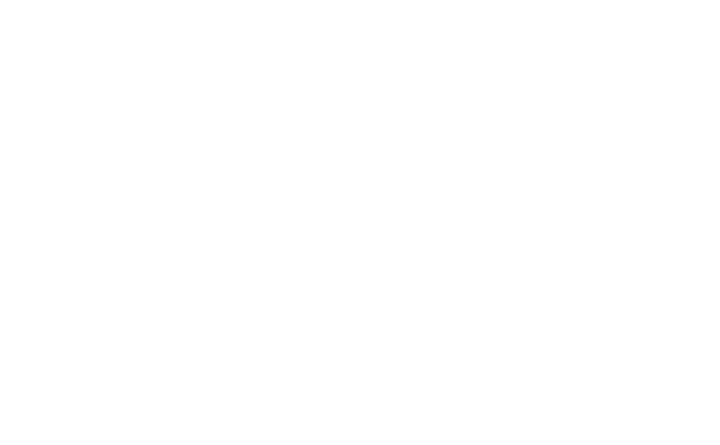
\includegraphics{Phase_Transition.png}
\end{document}